\documentclass[unicode]{beamer}

\usepackage[utf8]{inputenc}
\usepackage{cmap}
\usepackage[russian]{babel}

% listings
\usepackage{listings}
\lstset{language=java,frame=shadowbox,rulesepcolor=\color{gray},
        resetmargins=true,showstringspaces=false,
        basicstyle=\ttfamily,keywordstyle=\color{blue},
        stringstyle=\color{purple},commentstyle=\color{gray},
        morekeywords={assert,enum,@interface}}

% beamer
\usetheme{CambridgeUS}

\beamertemplatenavigationsymbolsempty

\setbeamertemplate{bibliography item}[book]
\setbeamertemplate{bibliography entry note}{//~}
\setbeamercolor{bibliography entry note}{fg=structure}


\title[Многопоточность (2)]{Многопоточность в Java:\\средства стандартной библиотеки}
\author{Алексей Владыкин}
\date{20 ноября 2017}

\begin{document}

\begin{frame}
\titlepage
\end{frame}

\begin{frame}
\tableofcontents
\end{frame}


\section{Атомарные типы}

\begin{frame}
\centering

\includegraphics[width=0.9\textwidth]{pics/atomic.jpg}

\underline{\url{http://en.wikipedia.org/wiki/A_Boy_and_His_Atom}}
\end{frame}


\begin{frame}
\begin{itemize}
\item Пакет \texttt{java.util.concurrent.atomic}
	\bigskip

\item \texttt{AtomicBoolean}\\
	\texttt{AtomicInteger}\\
	\texttt{AtomicLong}\\
	\texttt{AtomicReference<V>}
	\bigskip

\item Операции:\\
	\lstinline{V get()}\\
	\lstinline{void set(V newValue)}\\
	\lstinline{boolean compareAndSet(V expect, V update)}
\end{itemize}
\end{frame}


\begin{frame}[fragile]
\begin{itemize}
\item Примитив \texttt{compareAndSet} позволяет реализовывать другие операции
	\bigskip

\item Пример из \texttt{AtomicInteger}:
\end{itemize}
\begin{lstlisting}
public final int incrementAndGet() {
    for (;;) {
        int current = get();
        int next = current + 1;
        if (compareAndSet(current, next))
            return next;
    }
}
\end{lstlisting}
\end{frame}



\section{Примитивы синхронизации}

\begin{frame}
\centering
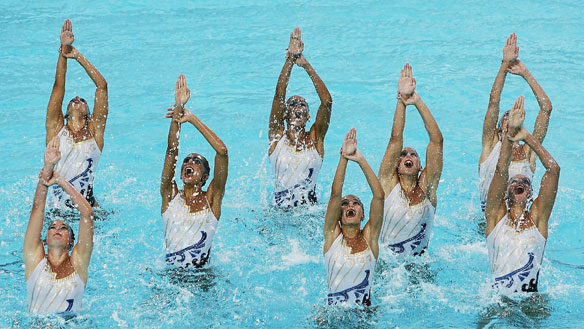
\includegraphics[width=0.9\textwidth]{pics/synchronization.jpg}
\end{frame}


\begin{frame}{Semaphore}
\begin{itemize}
\item Класс \texttt{java.util.concurrent.Semaphore}
	\bigskip

\item Ограничивает одновременный доступ к ресурсу
	\bigskip

\item В отличие от \lstinline{synchronized}-блока, одновременно
	могут работать несколько потоков (но не более заданного~N)
	\bigskip

\item Операции:\\
	\lstinline{void acquire()}\\
	\lstinline{void release()}
\end{itemize}
\end{frame}


\begin{frame}[fragile]
\begin{lstlisting}
Semaphore semaphore = new Semaphore(10);

semaphore.acquire();
try {
    // up to 10 threads may
    // execute this code concurrently
} finally {
    semaphore.release();
}
\end{lstlisting}
\end{frame}


\begin{frame}{CountDownLatch}
\begin{itemize}
\item Класс \texttt{java.util.concurrent.CountDownLatch}
    \bigskip

\item Обеспечивает точку синхронизации между N~потоками\\
    (несколько потоков могут дожидаться друг друга и потом стартовать
    одновременно)
    \bigskip

\item Операции:\\
    \lstinline|void await()|\\
    \lstinline|void countDown()|
\end{itemize}
\end{frame}


\begin{frame}[fragile]
\begin{lstlisting}
CountDownLatch latch = new CountDownLatch(10);

// this call blocks until latch.countDown()
// is called at least 10 times
latch.await();
\end{lstlisting}
\end{frame}


\begin{frame}{CyclicBarrier}
\begin{itemize}
\item Класс \texttt{java.util.concurrent.CyclicBarrier}
    \bigskip

\item Вариант \texttt{CountDownLatch}, допускающий повторное ожидание
\end{itemize}
\end{frame}


\begin{frame}{ReentrantLock}
\begin{itemize}
\item Класс \texttt{java.util.concurrent.locks.ReentrantLock}
    \bigskip

\item Обеспечивает взаимное исключение потоков,
    аналогичное \lstinline|synchronized|-блокам
    \bigskip

\item Операции:\\
    \lstinline|lock()|\\
    \lstinline|unlock()|
\end{itemize}
\end{frame}


\begin{frame}[fragile]
\begin{lstlisting}
Lock lock = new ReentrantLock();

lock.lock();
try {
    doSomething();
} finally {
    lock.unlock();
}
\end{lstlisting}
\end{frame}


\begin{frame}{Condition}
\begin{itemize}
\item Класс \texttt{java.util.concurrent.locks.Condition}
    \bigskip

\item Аналог wait/notify
    \smallskip

\item Привязан к Lock'у
    \smallskip

\item У одного Lock'а может быть много Condition'ов
\end{itemize}
\end{frame}


\begin{frame}[fragile]
\begin{lstlisting}
Lock lock = new ReentrantLock();
Condition condition = lock.newCondition();

lock.lock();
try {
    while (!conditionSatisfied()) {
        condition.await();
    }
} finally { lock.unlock(); }

// somewhere else in our program
lock.lock();
try {
    condition.signal();
} finally { lock.unlock(); }
\end{lstlisting}
\end{frame}


\begin{frame}{ReentrantReadWriteLock}
\begin{itemize}
\item Класс \texttt{java.util.concurrent.locks.ReentrantReadWriteLock}
    \bigskip

\item Поддерживает разделение доступа на чтение и на запись
\end{itemize}
\end{frame}


\begin{frame}[fragile]
\begin{lstlisting}
ReadWriteLock lock = new ReentrantReadWriteLock();

// somewhere in our program
lock.readLock().lock();
try {
    readOnlyOperation();
} finally {
    lock.readLock().unlock();
}

// somewhere else in our program
lock.writeLock().lock();
try {
    modifyingOperation();
} finally {
    lock.writeLock().unlock();
}
\end{lstlisting}
\end{frame}



\section{Коллекции}

\begin{frame}
\centering

\includegraphics[width=0.7\textwidth]{pics/collections.jpg}
\end{frame}


\begin{frame}
\begin{itemize}
\item Пакет \texttt{java.util.concurrent}
    \bigskip

\item Многопоточные варианты стандартных коллекций:\\
    \texttt{ConcurrentHashMap}\\
    \texttt{ConcurrentSkipListMap}\\
    \texttt{ConcurrentSkipListSet}\\
    \texttt{CopyOnWriteArrayList}\\
    \texttt{CopyOnWriteArraySet}
    \bigskip

\item Более эффективны, чем полностью синхронизованные коллекции\\
    \lstinline|java.util.Collections.synchronizedCollection()|
\end{itemize}
\end{frame}


\begin{frame}{ConcurrentLinkedQueue}
\begin{itemize}
\item Класс \texttt{java.util.concurrent.ConcurrentLinkedQueue<E>}
    \bigskip

\item Реализация очереди, поддерживающая одновременный доступ из
    многих потоков, при этом не использующая блокировки
    \bigskip

\item Операции:\\
    \lstinline|boolean offer(E e)|\\
    \lstinline|E poll()|\\
    \lstinline|E peek()|
\end{itemize}
\end{frame}


\begin{frame}{BlockingQueue}
\begin{itemize}
\item Интерфейс \texttt{java.util.concurrent.BlockingQueue<E>}
    \bigskip

\item Очередь, поддерживающая ограничение по размеру и операции ожидания
    \bigskip

\item Операции:\\
    \lstinline|void put(E e)|\\
    \lstinline|E take()|
    \bigskip

\item Реализации:\\
    \texttt{LinkedBlockingQueue}, \texttt{ArrayBlockingQueue}, \ldots
\end{itemize}
\end{frame}



\section{Executors}

\begin{frame}
\centering

\includegraphics[width=0.9\textwidth]{pics/executors.jpg}
\end{frame}


\begin{frame}
\begin{itemize}
\item Класс \texttt{java.util.concurrent.ExecutorService} и его соседи
    \bigskip

\item Инфраструктура для выполнения задач в несколько потоков
    \bigskip

\item Инкапсулирует создание потоков, организацию очереди задач,
    распределение задач по потокам
\end{itemize}
\end{frame}


\begin{frame}{ExecutorService}
\begin{itemize}
\item \lstinline|Future<?> submit(Runnable task)|
    \bigskip

\item \lstinline|<T> Future<T> submit(Callable<T> task)|
    \bigskip

\item \lstinline|void shutdown()|
    \bigskip

\item \lstinline|List<Runnable> shutdownNow()|
\end{itemize}
\end{frame}


\begin{frame}{Executors}
\begin{itemize}
\item Класс \texttt{java.util.concurrent.Executors}
    \bigskip

\item \lstinline|ExecutorService newSingleThreadExecutor()|
    \bigskip

\item \lstinline|ExecutorService newFixedThreadPool(int nThreads)|
    \bigskip

\item \lstinline|ExecutorService newCachedThreadPool()|
\end{itemize}
\end{frame}


\begin{frame}{ForkJoinPool}
\begin{itemize}
\item Класс \texttt{java.util.concurrent.ForkJoinPool}
    \bigskip

\item Вариант \texttt{ExecutorService}, в котором выполняющиеся
    задачи могут динамически порождать подзадачи
    \bigskip

\item Принимает на исполнение \texttt{ForkJoinTask}
\end{itemize}
\end{frame}


\section{Parallel Streams}

\begin{frame}
\begin{itemize}
\item \lstinline|stream.parallel()|
    \bigskip

\item Возвращает stream, дальнейшие операции в котором
    будут исполняться параллельно
    \bigskip

\item Надо следить за доступом к общим данным из
    передаваемых в stream операций
\end{itemize}
\end{frame}


\end{document}

